\chapter{Design}\label{cap:design}
Dopo aver stabilito quelli che sono i requisiti funzionali della piattaforma si procede con la fase di design, nella quale si definisce l'architettura del sistema, gli strumenti per il suo sviluppo e l'organizzazione dei dati utilizzando modelli concettuali.

\section{Architettura del sistema}
L'architettura software di un sistema rappresenta le decisioni di progettazione relative alla struttura e al comportamento generale del sistema. Tale struttura  \`e definita dagli stili architetturali implementati, i quali stabiliscono come l'interfaccia utente e il codice sorgente back-end sono organizzati~\cite{FordRichards}.

\subsection{Architettura three-tier}
Si vuole sviluppare una piattaforma che sia flessibile e facilmente aggiornabile, scalabile e manutenibile. Si \`e deciso perci\`o di adottare come architettura del sistema l'architettura three-tier in quanto essa permette di sviluppare applicazioni in diversi strati, i quali possono essere sviluppati, aggiornati e modificati in maniera indipendente tra loro.

L'architettura three-tier \`e un'architettura ti tipo $ n $-tier, nella quale sono presenti tre strati logici, con ogni strato che svolge un ruolo specifico all'interno dell'applicazione e che comunica solo con lo strato adiacente. La separazione dei compiti nelle architetture a pi\`u strati semplifica la creazione di ruoli e modelli di responsabilit\`a efficaci all'interno dell'architettura. I componenti all'interno di uno specifico livello hanno un ambito limitato, occupandosi solo della logica che appartiene a quel livello~\cite{FordRichards2}.

In un'applicazione three-tier sono presenti i seguenti strati:
\begin{itemize}
	\item Presentazione: interagisce con l'utente finale attraverso un'interfaccia grafica. Lo scopo di questo strato \`e quello di visualizzare ed ottenere le informazioni.
	\item Logica di business: si occupa di elaborare le informazioni ottenute dallo strato di presentazione e gestire le operazioni di accesso ai dati.
	\item Dati: ha il compito di archiviare, gestite e fornire i dati persistenti elaborati dall'applicazione.
\end{itemize}

\subsection{Single Page Application}
Le applicazioni web tradizionali rientrano nelle categoria delle ``Multi Page Application'' ossia applicazioni nelle quali ogni richiesta di una nuova pagina si traduce in una richiesta al server, il quale, dopo aver elaborato la richiesta, esegue il render della pagina e la restituisce al client. Si ha quindi che, ogni qual volta che si vuole cambiare pagina, verr\`a effettuato un refresh dell'applicazione nel browser e l'utente dovr\`a aspettare che la pagina venga interamente scaricata.

Per lo strato presentazione si \`e deciso quindi di sviluppare una ``Single Page Application'' (SPA) in quanto molto pi\`u performanti. In una SPA l'intera applicazione viene eseguita come una singola pagina web. Pi\`u precisamente, invece di scaricare e caricare una nuova pagina, vengono scaricati i dati e i componenti relativi alla pagina d'interesse e poi viene generata localmente nel browser la nuova pagina e collegata dinamicamente al DOM tramite JavaScript. Quindi non sono mai necessari aggiornamenti del browser~\cite{EmmitScott}. 

Dal punto di vista dell'architettura lo strato di presentazione viene rimosso dal server e gestito all'interno del browser. Il server, quindi, si comporta come se fosse un livello di servizio e il client interagisce con esso solo per lo scambio di dati.

\subsection{Web service}
Per lo strato di logica di business si \`e deciso di sviluppare un web service, o servizio web, ossia un sistema software progettato per supportare l'interazione da macchina a macchina interoperabile su una rete~\cite{webservicesarchitecture}. Nella pratica, i web service sono applicazioni web distribuite che espongono all'esterno le proprie funzionalit\`a e risorse tramite un'interfaccia che utilizza gli standard e i protocolli di rete, come HTTP, per comunicare con altre applicazioni.

\subsubsection{L'architettura Resource-Oriented}
L'obiettivo dei web service \`e, quindi, connettere i sistemi informativi e il ``Resource-Oriented architecture'' (ROA) definisce una serie di linee guida per supportare e implementare le interazioni all'interno di qualsiasi risorsa connessa. Ogni entit\`a logica di un'applicazione pu\`o essere rappresentata come una risorsa, identificata da una URI, e resa accessibile tramite l'utilizzo di metodi HTTP standard, quali GET, POST, PUT, PATCH e DELETE~\cite{SubramanianRaj}.

Inoltre il ROA presenta una serie di benefici considerevoli, in termini di caratteristiche dell'architettura, quali indipendenza del server dal cliente, scalabilit\`a e performance.

Lo stile ROA implementa i criteri di progettazione definiti nello stile architetturale ``REST'' (Representational State Transfer). Il termine REST  si riferisce ad un insieme di principi architetturali per la progettazione di sistemi distribuiti, e, in quanto tale, \`e molto generale. In particolare, non \`e legato al Web, nulla su REST dipende dai meccanismi di HTTP o dalla struttura degli URI. Per questo motivo si scegli uno stile ROA, il quale richiede espressamente l'uso di URI per identificare le risorse e l'utilizzo di metodi HTTP standard per l'interazione con le risorse, per lo sviluppo di web service di tipo RESTful~\cite{RichardsonRuby}. 

\subsubsection{Comunicazione tra SPA e Web service}
La comunicazione tra front-end, rappresentato dalla SPA, e back-end, rappresentato dal web service, avverr\`a tramite una RESTful API (Application Programming Interface) esportata dall'applicazione back-end. Tale comunicazione parte dal front-end, il quale effettua richieste HTTP verso l'API RESTful del back-end. L'API RESTful esegue quindi le operazioni richieste e restituisce una risposta, in formato JSON, al front-end.

Per le rispose del web service si \`e scelto di utilizzare lo standard JSend, il quale prevede tre tipologie di risposta: successo, fallimento ed errore~\cite{JSend}.

\subsection{Gestione dati persistenti}
Per la gestione dei dati persistenti si \`e deciso di utilizzare un ``Database Management System'' (DBMS), ossia un sistema software in grado di definire, creare, mantenere e controllare collezioni di dati grandi, condivise e persistenti, in maniera efficiente e sicura. Pi\`u precisamente si \`e deciso di adottare un ``Relational DataBase Management System'' (RDBMS) ossia un DBMS basato sul modello relazionale, nel quale i dati sono organizzati in record di dimensione fissa, e divisi in tabelle, dette relazioni.

La scelta del RDBMS da adottare \`e ricaduta sul RDBMS open-source MySQL, sviluppato da Oracle e basato sul linguaggio ``Structured Query Language'' (SQL).
\section{Framework}
I framework sono sistemi composti da un insieme di strumenti e librerie progettati per migliorare la qualit\`a del software sviluppato. Essi forniscono, inoltre, convenzioni che riducono la quantit\`a di codice che uno sviluppatore nuovo al progetto deve comprendere.

Si distinguono tre tipologie di framework per la realizzazione di applicazioni web:
\begin{itemize}
	\item Back-end: facilita lo sviluppo lato server, fornendo gli strumenti per la gestione del database, della business logic e delle richieste al server.
	\item Front-end: facilita lo sviluppo lato client, fornendo gli strumenti per la creazione e l'accesso delle pagine, gestendo inoltre le interazioni con l'utente.
	\item User Interface: facilita lo sviluppo dell'aspetto visivo dell'applicazione.
\end{itemize}

\subsection{Back-end}
Per la parte back-end si \`e scelto ``Laravel'', un framework di sviluppo web MVC scritto in PHP. Attualmente si trova alla versione 9.

Laravel permette uno sviluppo rapido di applicazioni web, in quanto ha una bassa curva di apprendimento e fornisce una serie di componenti atti a facilitare tutte le attivit\`a pi\`u comuni nella creazione di applicazioni web, come l'interazioni del database, l'autenticazione, la gestione della posta elettronica e la memorizzazione nella cache~\cite{Stauffer}. 

Un ulteriore punto di forza di Laravel \`e dato dai diversi strumenti che fornisce per lo sviluppo di RESTful API. Sono infatti presenti meccanismi per gestire e proteggere le route dell'API, validare le richieste e formattare e restituire le risposte in formato JSON. 
\subsubsection{Laravel Sanctum}
Laravel Sanctum \`e un pacchetto che fornisce un sistema di autenticazione, basato su token, facile e leggero. Sanctum consente a ciascun utente di un applicazione di generare uno o pi\`u Bearer Token per il proprio account. I Bearer Token sono una particolare tipologia di access token usati per ottenere l'autorizzazione ad accedere alle risorse protette dell'applicazione.
\subsection{Front-end}
Per lo sviluppo della SPA si \`e scelto `` Vue.js'', un framework front-end JavaScript open-source ideale per lo sviluppo di interfacce web e SPA. Attualmente alla versione 3, Vue.js \`e un framework leggero, con un peso di circa 24 KB, veloce, flessibile e facile da usare.

Vue.js combina gli aspetti e i principi pi\`u utili e innovativi degli altri framework JavaScript come la gestione dello stato applicativo, l'utilizzo di un DOM virtuale, il routing e l'utilizzo di pattern MVVM per sparare il codice HTML da quello JavaScript~\cite{HanchettListwon}. Un'altra importante caratteristica di Vue.js \`e l'abilita di creare ed utilizzare elementi HTML personalizzati chiamati componenti, ossia istanze Vue riutilizzabili con elementi HTML personalizzati.
\subsubsection{Pinia}
Pinia \`e la libreria per la gestione dello stato ufficialmente suggerita per Vue.js. Essa sostituisce la libreria Vuex, utilizzata per la gestione dello stato nelle precedenti versioni di Vue.js.

Per stato si intende l'insieme dei dati utilizzati all'interno dell'applicazione, e la sua gestione consiste nella possibilit\`a di condividere e modificare tale stato tra le varie pagine e tra i componenti dell'applicazione.

Le caratteristiche principali di Pinia sono la facilit\`a con la quale \`e possibile creare ed utilizzare gli store per la gestione dello stato e la sua modularit\`a che permette di avere pi\`u store simultaneamente.

\subsection{User interface}
L'interfaccia utente verr\`a realizzata utilizzando il framework CSS ``Tailwind CSS''.

Tailwind CSS si differenzia da altri framework CSS in quanto si pone ad un livello pi\`u basso, fornendo delle classi di utility per realizzare design personalizzati invece di componenti preconfezionati.

\section{Database}
Una volta raccolti e definiti tutti i requisiti della piattaforma e identificate le tecnologie per il back-end \`e possibile procedere con la fase di progettazione della base di dati, nella quale, attraverso l'utilizzo di modelli concettuali, si individua la struttura e l'organizzazione che i dati dovranno avere.

In questa sezione del capitolo viene riportato la progettazione concettuale della base di dati, la quale viene rappresentato utilizzando i diagrammi delle classi UML.

\subsection{Utente}
Dalla raccolta dei requisiti relativi all'autenticazione e alle impostazioni \`e emerso che:
\begin{itemize}
	\item Per ogni utente si devono memorizzare nome, username, indirizzo e-mail e password.
	\item Lo username deve essere un attributo unico in quanto permette di identificare univocamente l'utente all'interno piattaforma.
	\item L'e-mail deve essere un attributo unico in quanto viene utilizzata come credenziale d'accesso.
	\item L'indirizzo e-mail dell'utente deve essere verificato.
	\item L'utente deve per poter gestire l'immagine di profilo.
	\item \`E possibile ripristinare il proprio account dopo averlo eliminato.	
\end{itemize}

Si ricava quindi la classe ``users'':
\begin{figure}[htbp]
	\centering
	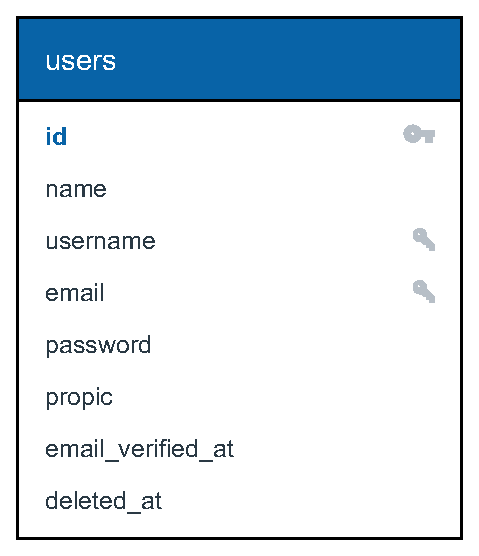
\includegraphics[height=0.35\linewidth]{figure/users_db}
	\caption{Rappresentazione UML dell'utente}
	\label{fig:users_db}
\end{figure}

\subsection{Portfolio}
Dalla raccolta dei requisiti relativi al portfolio \`e emerso che:
\begin{itemize}
	\item Ogni utente pu\`o gestire al pi\`u un portfolio.
	\item Per ogni portfolio si deve memorizzare il nome.
	\item L'utente deve poter gestire l'icona del portfolio.
	\item Un portfolio pu\`o essere archiviato.
	\item \`E possibile ripristinare il proprio portfolio dopo averlo eliminato.
	\item Un portfolio \`e costituito da varie sezioni.
\end{itemize}

Le sezioni del portfolio permettono la navigazione all'interno del portfolio a cui appartengono. Tenendo in considerazione i requisiti relativi alle gallerie, ogni sezione:
\begin{itemize}
	\item Avr\`a un nome che deve essere unico per identificare univocamente la sezione all'interno del portfolio.
	\item Avr\`a  slug che deve essere unico per l'accesso alla sezione tramite URL.
	\item Avr\`a  categoria per gestire le diverse tipologie di sezioni.
	\item Potr\`a essere archiviata o eliminata.
\end{itemize}

Si ricavano quindi le classi ``portfolios'', ``sections'' e ``section\_categories'' (Figura~\ref{fig:portfolio_db}).

\begin{figure}[htbp]
	\centering
	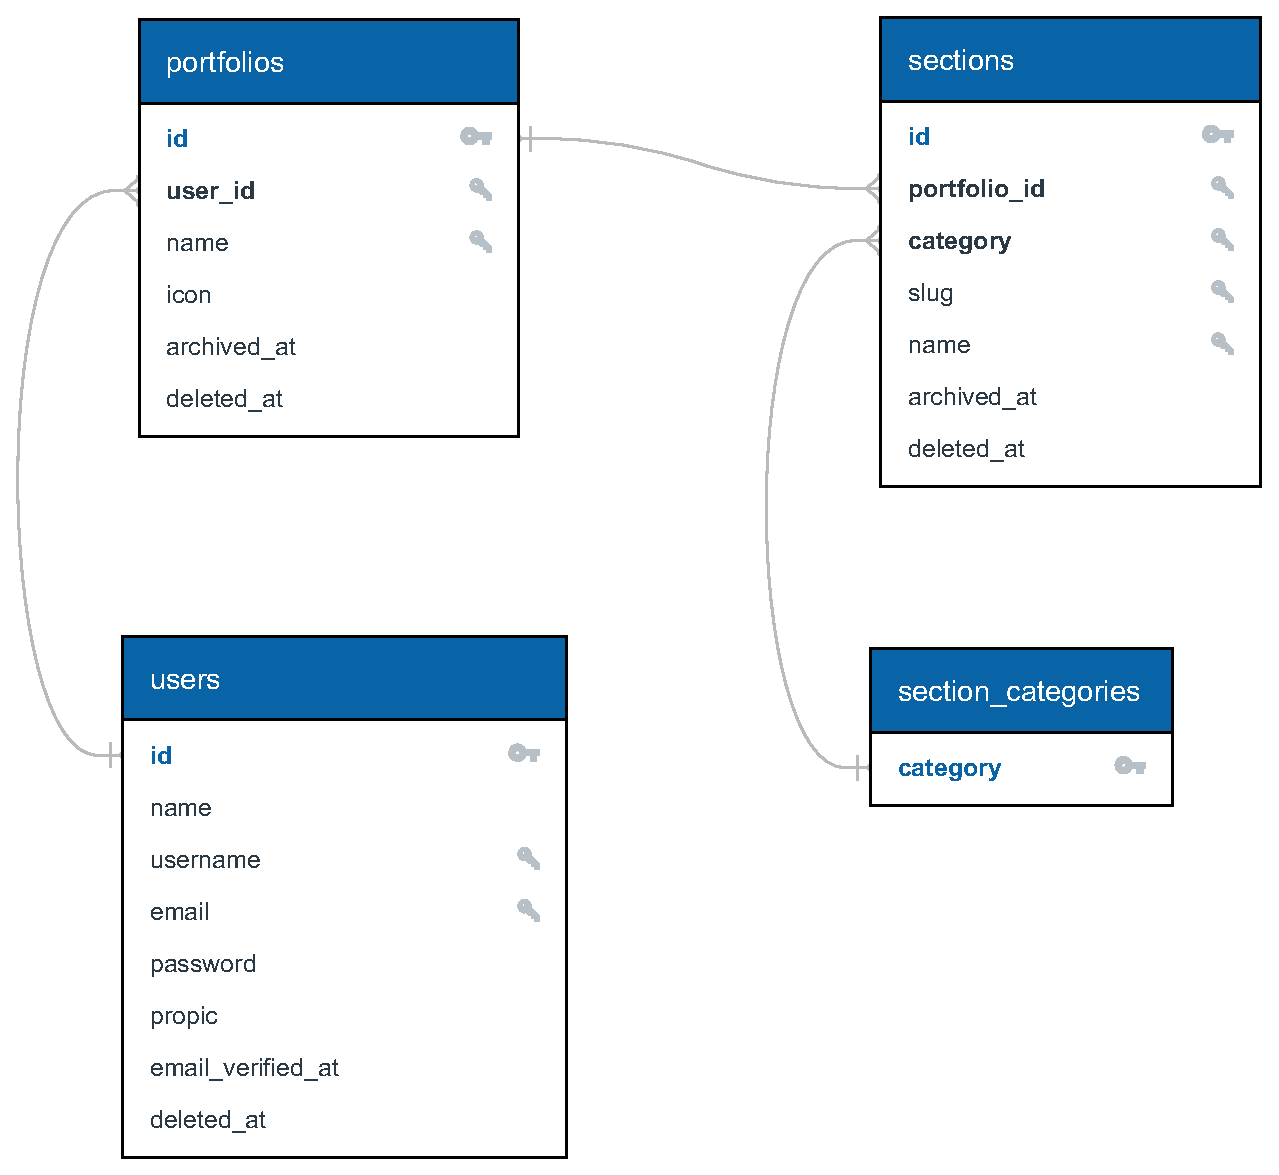
\includegraphics[width=0.8\linewidth]{figure/portfolio_db}
	\caption{Rappresentazione UML del portfolio e relative associazioni}
	\label{fig:portfolio_db}
\end{figure}

\subsection{Gallerie}
Dalla raccolta dei requisiti relativi alle gallerie \`e emerso che:
\begin{itemize}
	\item Ogni galleria appartiene ad una singola sezione.
	\item Per ogni galleria si vuole memorizzare una descrizione.
	\item L'utente pu\`o stabilire la posizione delle gallerie nella barra di navigazione del proprio portfolio.
	\item Ogni galleria ha dei post.
\end{itemize}

Si ricava quindi la classe ``galleries'' (Figura~\ref{fig:galleries_db}).

\begin{figure}[htbp]
	\centering
	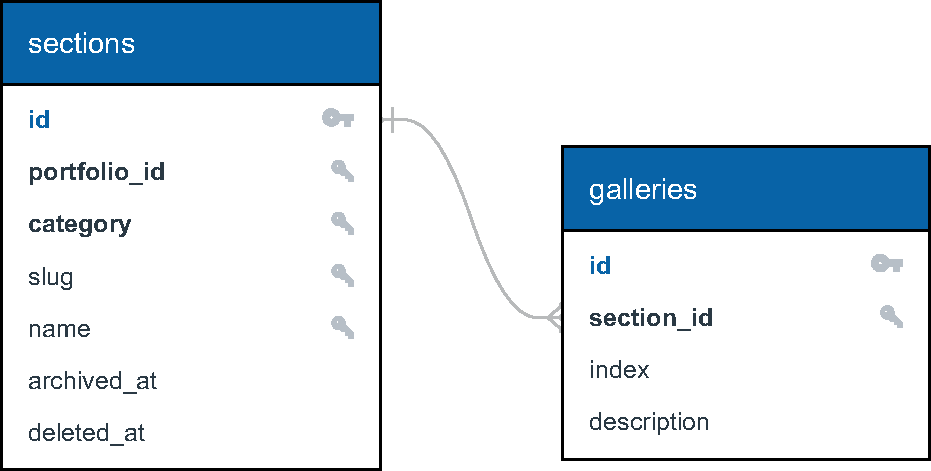
\includegraphics[width=0.76\linewidth]{figure/galleries_db}
	\caption{Rappresentazione UML della galleria e relativa associazione}
	\label{fig:galleries_db}
\end{figure}

\subsection{Post}
Dalla raccolta dei requisiti relativi ai post \`e emerso che:
\begin{itemize}
	\item Ogni post appartiene ad una galleria.
	\item Per ogni post si vuole memorizzare un titolo ed una descrizione.
	\item Ogni post \`e costituito da un media.
\end{itemize}

Inoltre, ogni post sar\`a identificato da uno slug unico.

Si ricava quindi la classe ``posts'' (Figura~\ref{fig:posts_db}).
\begin{figure}[htbp]
	\centering
	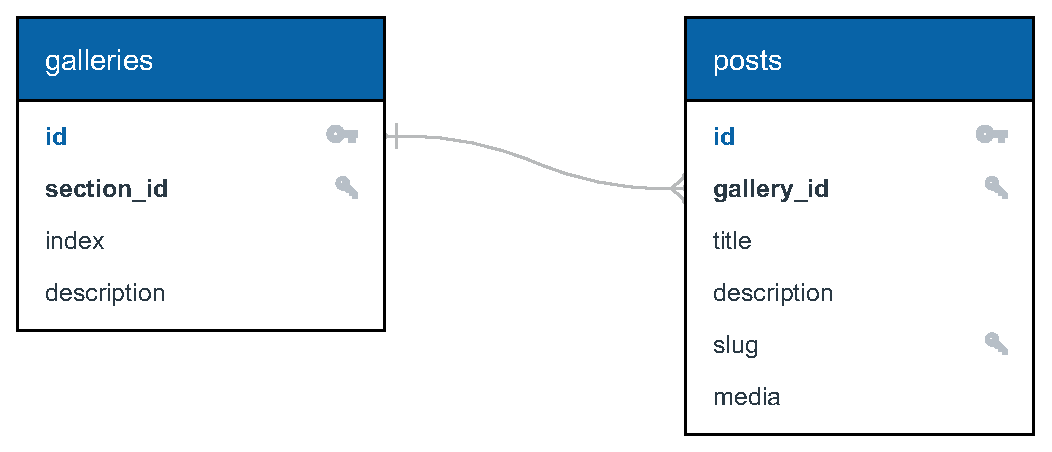
\includegraphics[width=0.76\linewidth]{figure/posts_db}
	\caption{Rappresentazione UML del post e relativa associazione}
	\label{fig:posts_db}
\end{figure}

\subsection{About me}
Dalla raccolta dei requisiti relativi alla sezione ``About me'' \`e emerso che:
\begin{itemize}
	\item Ogni portfolio ha una sezione per la presentazione dell'utente.
	\item Per la presentazione si vuole memorizzare una descrizione ed un indirizzo e-mail.
\end{itemize}

Si ricavano quindi le classi ``biographies'' e ``contacts'' (Figura~\ref{fig:about_me_db}).
\begin{figure}[H]
	\centering
	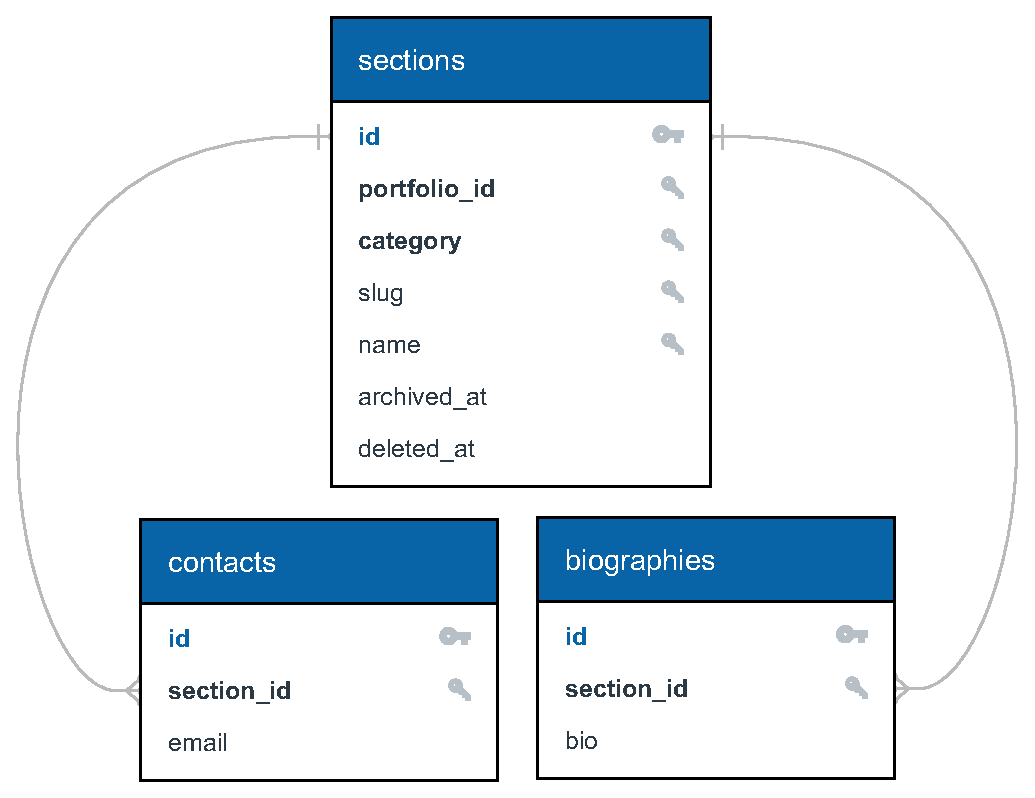
\includegraphics[width=0.7\linewidth]{figure/about_me_db}
	\caption{Rappresentazione UML del contenuto della sezione ``about me'' e relativa associazione}
	\label{fig:about_me_db}
\end{figure}

\subsection{Modello concettuale finale}
Dalla progettazione concettuale della base di dati si ricava il modello concettuale in Figura~\ref{fig:db}.

\begin{sidewaysfigure}[htbp]
	\centering
	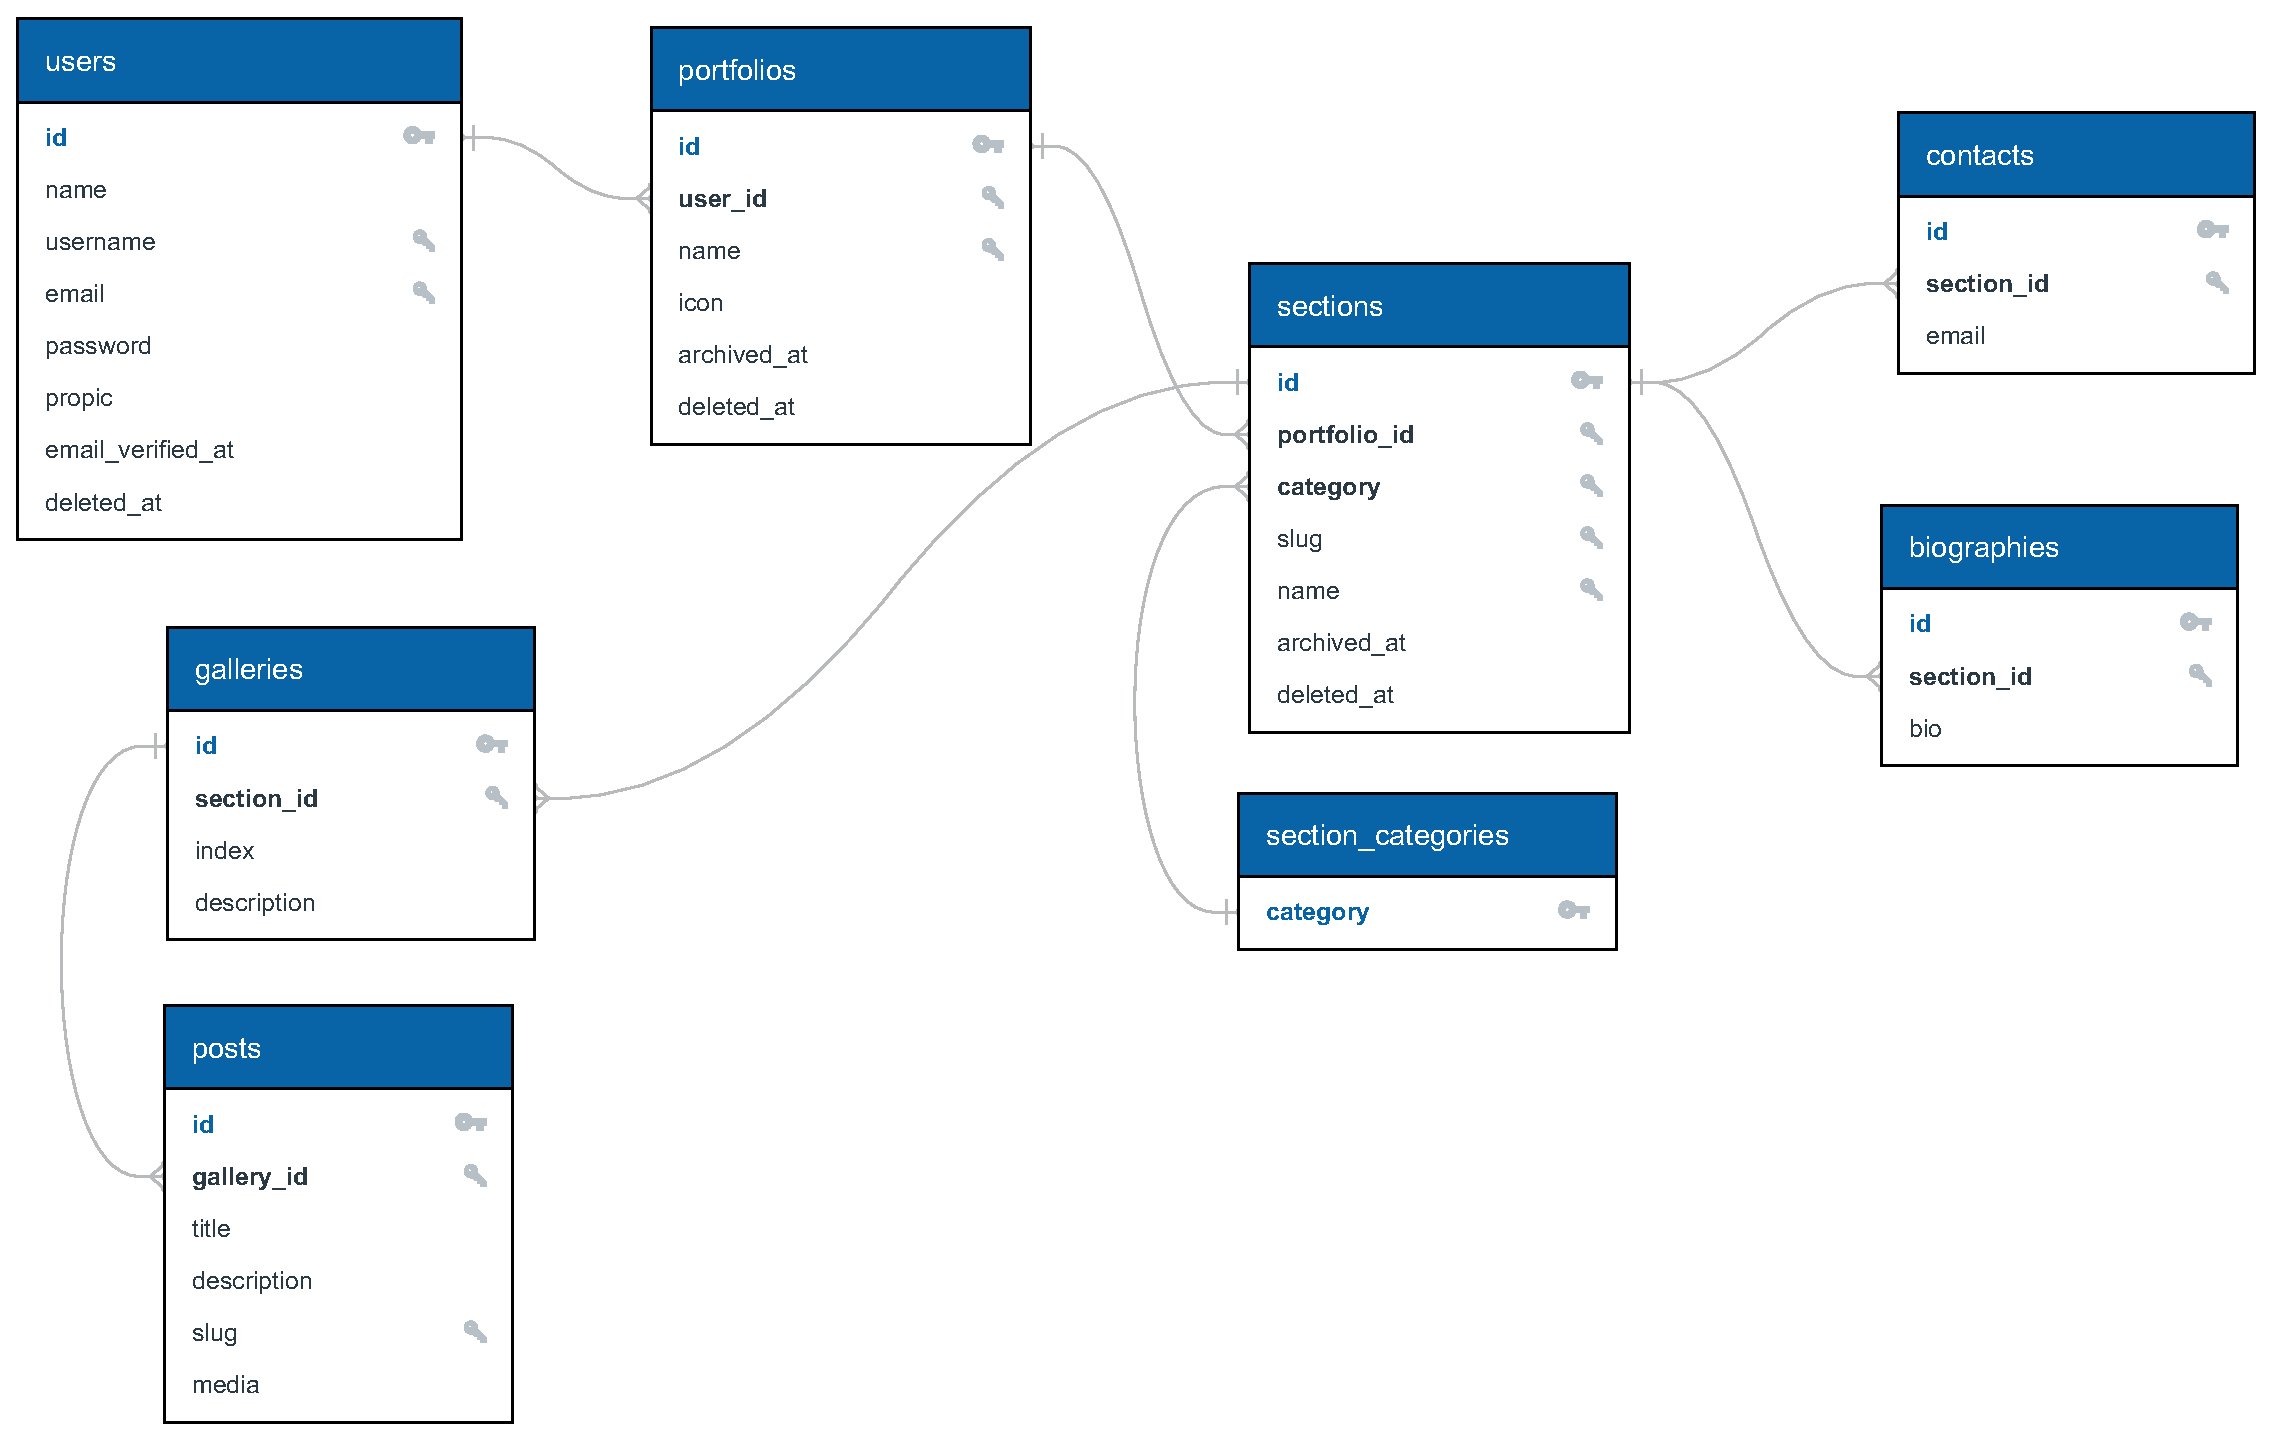
\includegraphics[width=0.9\linewidth]{figure/db}
	\caption{Modello concettuale finale}
	\label{fig:db}
\end{sidewaysfigure}


